\documentclass[aspectratio=169,10pt]{beamer}
\usetheme{Madrid}\usecolortheme{default}
\usepackage[T1]{fontenc}\usepackage{lmodern,booktabs,graphicx}
% Primary palette from the supplied main.tex.
\definecolor{B}{HTML}{08357E}
\definecolor{b}{HTML}{3C78D8}
\definecolor{g}{HTML}{38761D}
\definecolor{r}{HTML}{7A0101}
\definecolor{R}{HTML}{CE8F89}
\definecolor{P}{HTML}{5A43A0}
\definecolor{o}{HTML}{FF7F0E}

\setbeamercolor{structure}{fg=B}\setbeamercolor{frametitle}{fg=white,bg=B}
\setbeamercolor{block title}{fg=white,bg=B}\setbeamercolor{block body}{bg=b!7}
\setbeamercolor{alerted text}{fg=r}\setbeamertemplate{navigation symbols}{}\setbeamertemplate{footline}[frame number]
\title{Power-board battery case}\author{MIT Rocket Team Simulations}\date{9 November 2026}
\begin{document}
\begin{frame}{A flush case intersects all three cells before tightening}
\begin{columns}[T,onlytextwidth]\column{.56\textwidth}
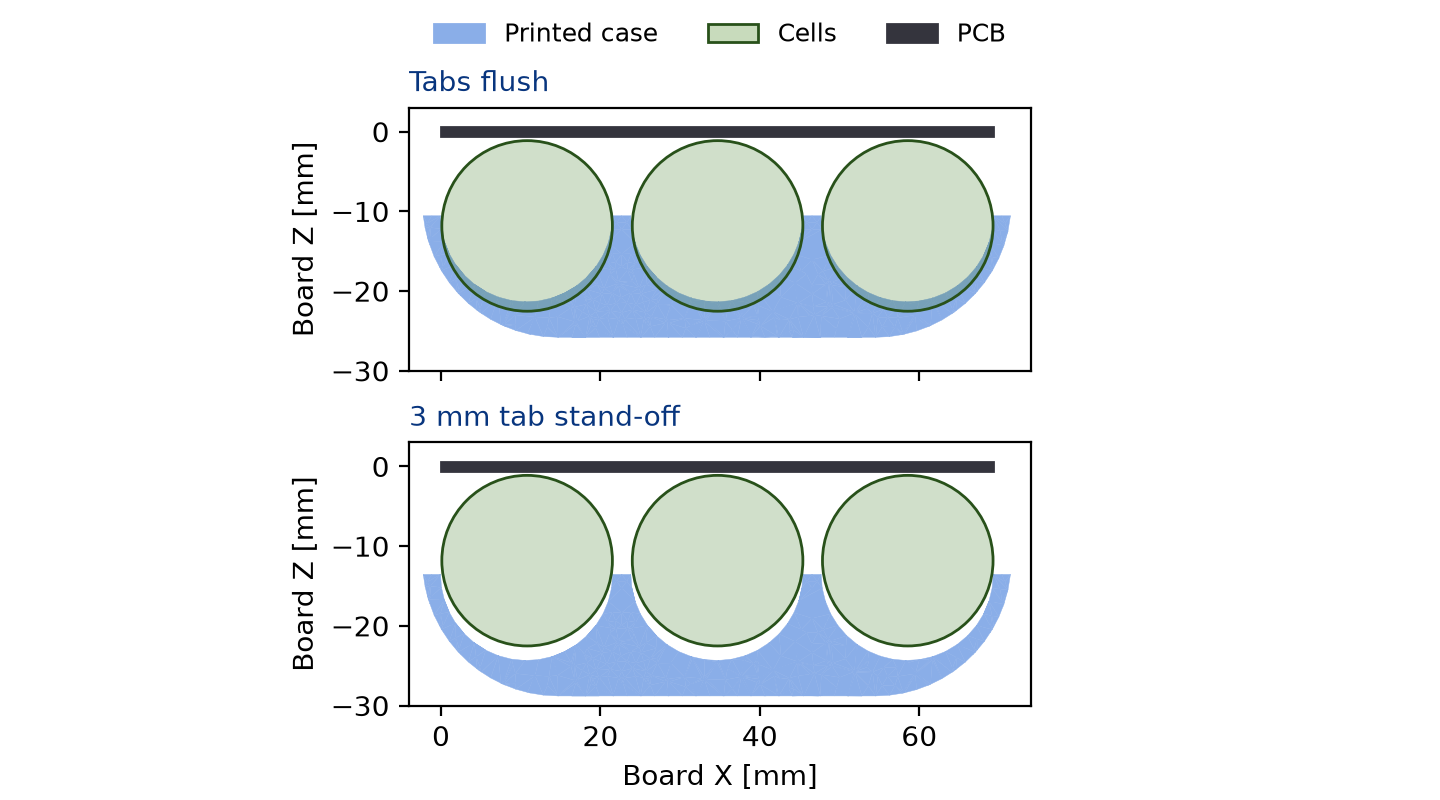
\includegraphics[width=\linewidth]{figures/midspan-fit.png}
\column{.41\textwidth}
\textbf{Flush tabs}\par Each cell overlaps the printed case by 1.18~mm at its crown. The local nylon-screw solve reached 2.87 of 3.00~mm drawdown. All four tabs crossed the modeled board plane, leaving the physical seating load unresolved.
\vspace{6mm}\par\textbf{3 mm stand-off}\par The unstrained STEP clears the cells and all existing mechanical hardware. Rigid sideways travel of 0.15--0.33 mm closes the first cell gap.
\end{columns}
\vfill{\footnotesize\color{B}Power-board geometry review\quad|\quad 8 November 2026}
\end{frame}
\begin{frame}{The hole pattern leaves little room for an M4 screw}
\begin{columns}[T,onlytextwidth]\column{.55\textwidth}
\begin{tabular}{lrr}\toprule & PCB & Case\\\midrule
Bore diameter [mm] &4.200&5.000--5.090\\
Hole pitch X [mm] &62.865&62.855\\
Hole pitch Y [mm] &114.427&113.241\\\bottomrule
\end{tabular}
\vspace{5mm}\par Each end of the centred pattern is about 0.593 mm off-axis. The smaller bore pair allows 0.600 mm with a nominal M4 shank.
\column{.41\textwidth}
\textbf{Hardware under study}\par Four M4 case screws in aluminium or nylon. The nylon reference is McMaster-Carr 93640A145.
\vspace{5mm}\par The dense PLA case adds about 74 g to a 252 g bare assembly. Print orientation and infill affect its installed stiffness and mass.
\end{columns}
\end{frame}
\begin{frame}{The bare-board preload repeats the October baseline}
\begin{tabular}{p{.51\textwidth}rp{.19\textwidth}}\toprule
Bare-board quantity & Value & Loading\\\midrule
First prestressed natural frequency & 485.964 Hz & Six bolts locked\\
Maximum PCB directional displacement & 0.052674 mm RMS & Base Z\\
Maximum PCB equivalent stress & 90.325 MPa RMS & Base X\\\bottomrule
\end{tabular}
\vspace{4mm}\par The fresh six-bolt solve held 749.997--749.999 N at each locked fastener and reproduced the October peak static displacement of 0.04746~mm. The fresh native X vibration run also reproduced the October PCB stress of 90.325~MPa RMS.
\vspace{3mm}\par\small The fresh bare edge-cell fixture took 8.54 N to reach 0.50 mm sideways travel. The raised case with nylon screws is the first cased comparison.
\end{frame}
\begin{frame}{The raised nylon-screw case restrains the edge cell}
\begin{columns}[T,onlytextwidth]
\column{.55\textwidth}
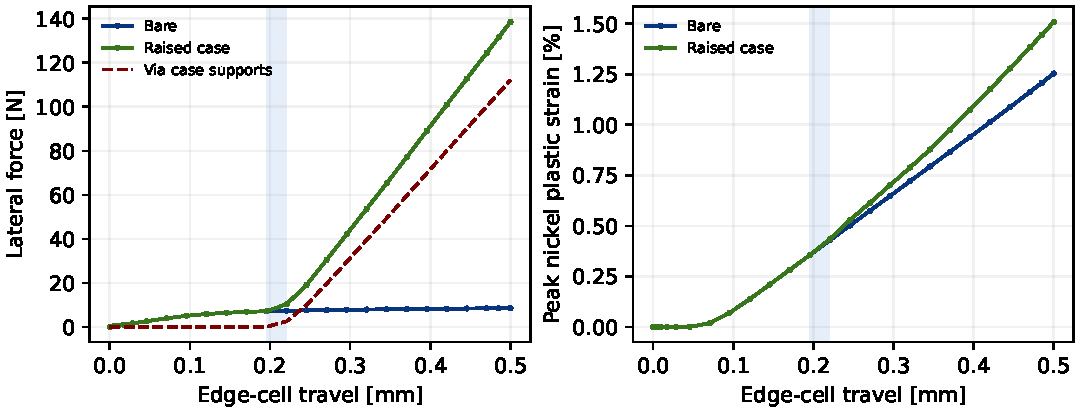
\includegraphics[width=\linewidth]{figures/stand3_nylon_lateral_friction_locked_pin1.pdf}
\par\small The blue band brackets first contact at 0.196--0.221~mm of travel.
\column{.42\textwidth}
\textbf{At the same 8.54 N pull}\\
Cell travel fell from 0.50 mm to about 0.21 mm. Peak nickel plastic strain was 1.25\% bare; the two cased states bracketing 8.54 N gave 0.36\% and 0.43\%.
\vspace{3mm}\par\textbf{At the same 0.50 mm travel}\\
The pull rose from 8.54 to 138.53 N. The four case screw supports carried 112.15 N. Peak nickel plastic strain rose from 1.25\% to 1.51\%.
\end{columns}
\vfill{\footnotesize\color{B}Local fixture, 3 mm stand-off, positive X pull with fixed screw tops.}
\end{frame}
\begin{frame}{Aluminium screws further reduced PCB deflection during tightening}
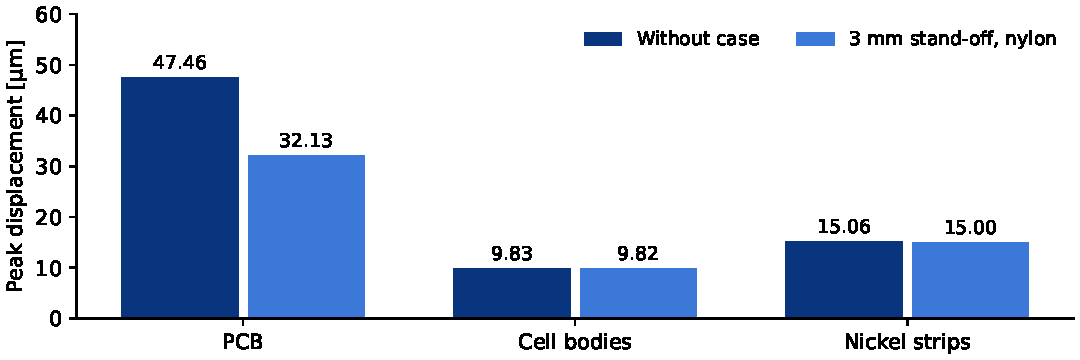
\includegraphics[width=.76\linewidth]{figures/raised-static-comparison.pdf}
\vspace{1mm}\par The same PCB node moved 47.46~$\mu$m bare, 32.13~$\mu$m with nylon screws and \textbf{27.13~$\mu$m} with aluminium screws. The reductions from bare were 32\% and 43\%, respectively.
\vspace{2mm}\par No cell, strip or washer contacted the case during tightening. Load transfer was through the four corner attachments.
\vfill{\footnotesize\color{B}3 mm stand-off. Six original bolts loaded to 750 N each and locked. No imposed vibration.}
\end{frame}
\begin{frame}{Both raised cases introduce modes below 486 Hz}
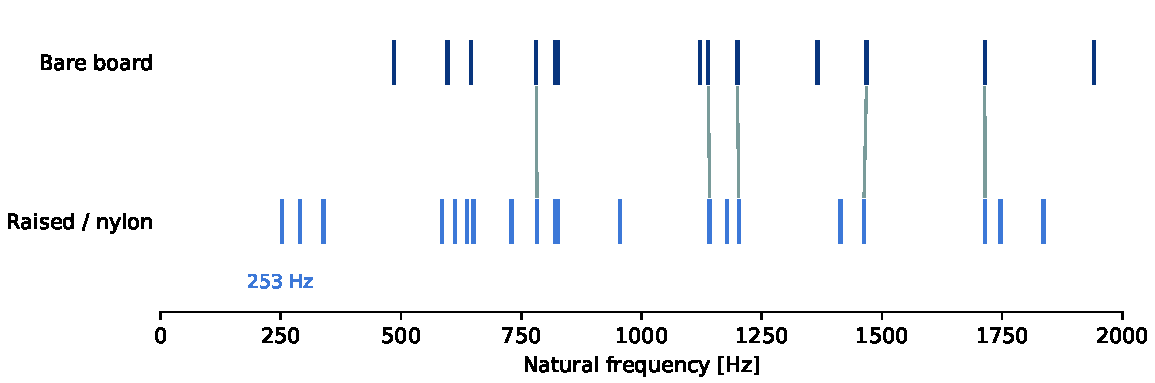
\includegraphics[width=.83\linewidth]{figures/raised-prestressed-modes.pdf}
\par The first cased mode rises from \textbf{253 Hz with nylon} to \textbf{320 Hz with aluminium}. Its shape remains closely matched across 399,194 solid nodes (MAC 0.989).
\vspace{2mm}\par The 781 Hz bare battery-motion mode reappears at 783 Hz with the case (shape correlation 0.943). Comparing modes by rank alone would miss this match.
\vfill{\footnotesize\color{B}Bolt-locked flexible assemblies at 3 mm stand-off. Undamped mode shapes about the tightened state.}
\end{frame}
\begin{frame}{The open-gap vibration model predicts more PCB motion}
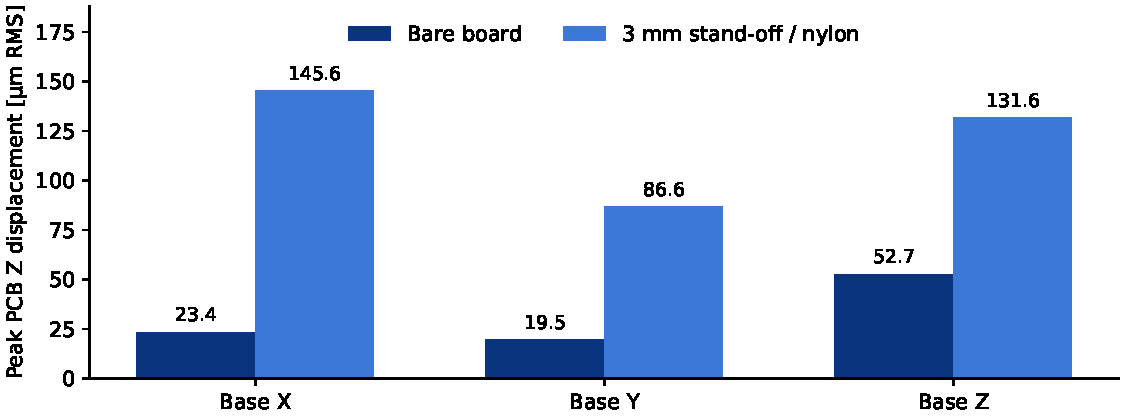
\includegraphics[width=.79\linewidth]{figures/raised-independent-psd.pdf}
\par With base X excitation, peak PCB Z motion was \textbf{23.37}~$\mu$m RMS bare, \textbf{145.55} with nylon and \textbf{120.00} with aluminium. The figure uses independent modal integration.
\vspace{2mm}\par\small Native MAPDL confirms both base-X results. Aluminium reduced board motion relative to nylon, but raised peak stress across the PLA layers near a screw bearing from 17.16 to 24.78 MPa RMS. Both raised models reached cell contact in the seeded motion.
\end{frame}
\end{document}
